\documentclass[a4paper]{article}

\usepackage{INTERSPEECH2018}
\usepackage{booktabs}
\usepackage{adjustbox}
\usepackage{multirow}
\usepackage{textcomp}

\title{Multilingual Multi-Task Learning for Low-Resource Acoustic Modeling}

\name{Josh Meyer$^1$}
%The maximum number of authors in the author list is twenty. If the number of contributing authors is more than twenty, they should be listed in a footnote or in acknowledgement section, as appropriate.
\address{
  $^1$University of Arizona}
\email{joshua.richard.meyer@gmail.com}

\begin{document}

\maketitle
% 
\begin{abstract}
  
\end{abstract}
\noindent\textbf{Index Terms}: speech recognition, multi-task learning, acoustic modeling

\section{Introduction}

Previous work has shown that performance for a low-resource language on speech recognition can be improved by adding training data from another, resource-rich language. Typically, data from another language is added as a separate task in the Multi-Task Learning framework via an additional output layer (Caruana 1997).

The targets for this addititional language have always been states of context-dependent triphones, defined by some tree clustering algorithm. This current research builds off the intuition that triphones encode information which is too fine-grained to be maximally useful for language-transfer. Using a higher-level of linguistic abstraction (eg. the monophone), we are able to better extract the kind of language-general information useful in training an acoustic model for some target language.

The intuition being that when adding a source language as an auxialilary task, it would be better to focus on source-language distinctions which are robust and will transfer well to a new, target language.

Each auxiliary task is created by redefining the parameters of the HMM-GMM system used to bootstrap a DNN-hybrid system, such that the phonetic decision tree is cut short.

The target language is Kyrgyz, and the source language is English. Both data come from audiobooks, English being from LibriSpeech and Kyrgyz from the Bizdin.kg project.




\section{Background Literature}




Mohan \& Rose 2015 ICASSP

Mostly they improve memory efficiency... use senomes.

\textit{  A relative improvement of 8.9\% was
observed with the multi-lingual DNN system over the mono-lingual
hybrid DNN-HMM system on the German evaluation set. To reduce
computational complexity, a low-rank matrix factorization (LRMF)
of the weight matrices in the final layer was proposed.}





Huang etal 2015 Interspeech Rapid Adaptation for Deep Neural Networks through Multi-Task Learning:

Monolingual (WSJ) -- looking at adaptation techniques

\textit{auxiliary output layers modeling
broad acoustic units, such as mono-phones or tied-state (often
called senone) clusters.}




Seltzer Droppo 2013:

Multitask TIMIT with three aux tasks:

\textit{. In the first system,
prediction of the phoneme identity is used as the secondary task.
This enables acoustic states to learn which acoustic states may be
similar via their shared common source phone. The second system
uses the previous and subsequent acoustic states as secondary tasks,
which informs the network about the temporal evolution of the la-
bels. Finally, the third proposed system uses the prediction of left
and right phonetic context as the secondary tasks. This enables the
network to learn about context dependency during training, while
still using simple context-independent acoustic model in decoding}




Chen, Mak, Leung, Sivadas 2014

Low-resource MTL (no source language)

\textit{we try to improve the phonetic models of a low-resource language by using only its own language resources without relying on finding a good mapping between its phonemes and phonemes from other languages which is sometimes not easily achieved.}


Grezl and Karafiat (2017)

Using single Source Language.

More states == better (i think that's because more states is a harder task, and doesn't overfit as fast)

\textit{In this paper, we analyze the feasibility of using single well-resourced language – English – as a source language for multilingual techniques in context of Stacked Bottle-Neck tandem system.}



Multilingual DNN: Heigold 2013 et al.

Multi-task, but only triphones.

\textit{Experiments were performed for eleven Romance languages with a total amount  of  10k  hours  of  data.}

\section{DNN-Hybrid Training as Model Transfer}

The standard DNN-Hybrid approach requires the GMM-HMM system to provide the labels for supervised training. This reliance of the DNN on GMM alignments is actually a form of model transfer, where the DNN is trained to perform the extact same classification as its GMM predecessor. The DNN not only learns the frame alignments from the individual GMMs, but also the DNN indirectly learns the structure of the phonetic decision tree used to define the tied-state system. This is because the output layer of the DNN is trained to predict targets which were defined via leaves of the decision tree.


\begin{figure}[!htb]
  \centering
\minipage{0.5\textwidth}
  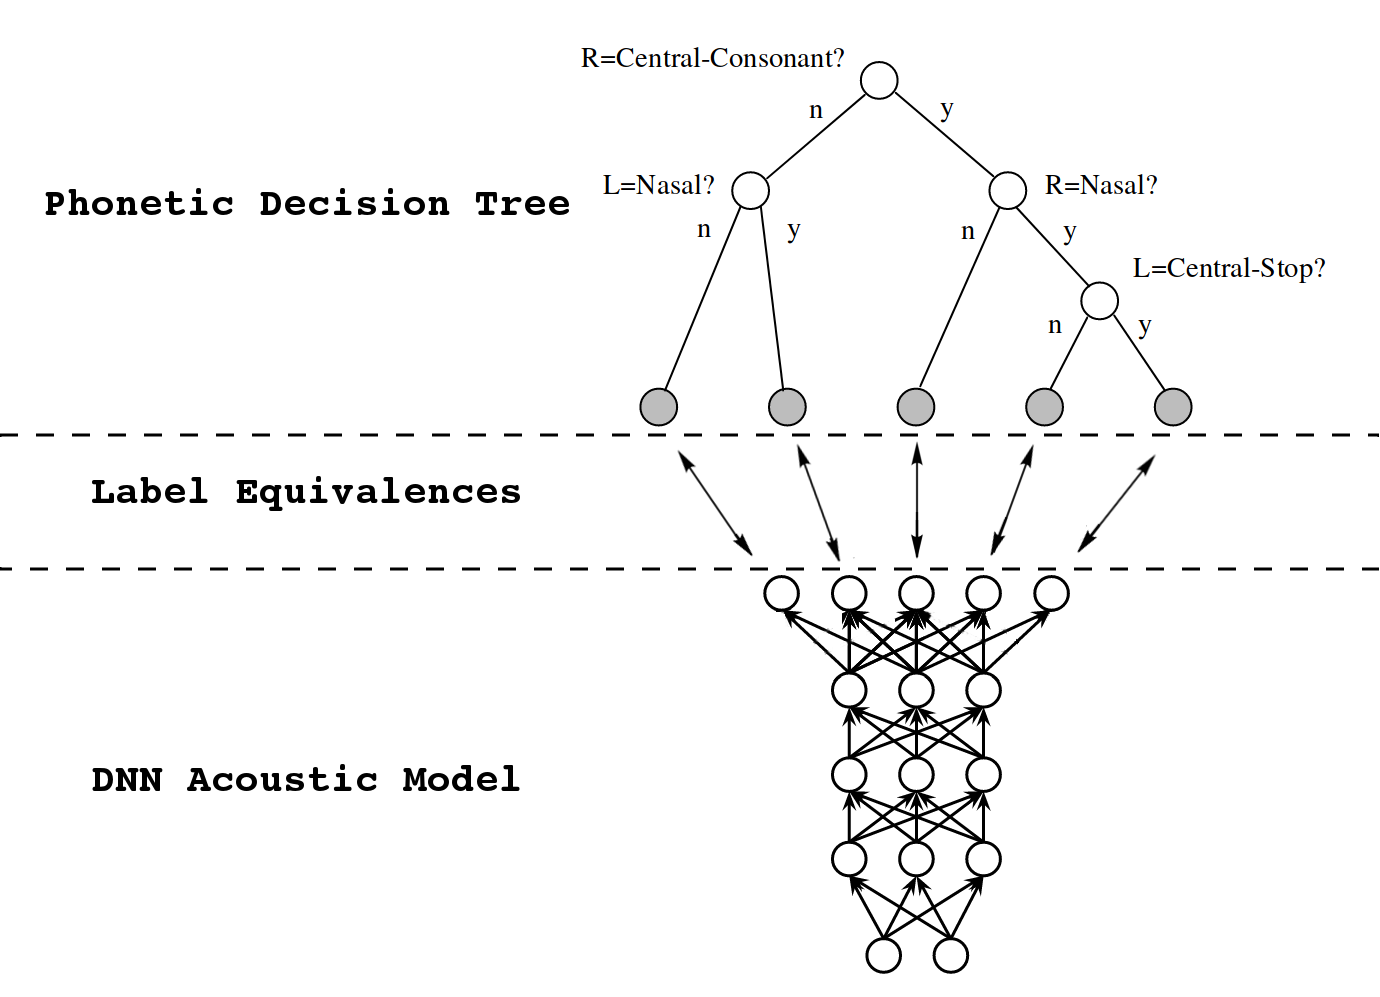
\includegraphics[width=\linewidth]{figs/tree-net.png}
  \caption{GMM$\rightarrow$DNN Model Transfer}
\endminipage\hfill
\end{figure}


Given that standard triphones encode very fine-grained information which may not help performance on a target language, the following experiments investigate GMM$\rightarrow$DNN model transfer at a higher level for an additional source language. 


\section{Experiments}

This work investigates the application of MTL technique to low resource acoustic modeling. All experiments relate to simulate a common development scenario: there exists little transcribed data for the target language, but lots of data in some source language.

The following experiments tease out (1) the level of detail at which the source language should be modeled and (2) the amount of weighting which should be given to the target language training examples.

The first point of interest: level of detail at which the source language should be modeled. This is investigated via addition of multiple tasks to the TDNN during backprop. Intuitively, we can model the source language with lots of contextual detail (ie. the triphone), with abstracted, context-independent detail (ie. the monophone), or somewhere in between (ie. the half-phone). Given the traditional ASR training pipeline, investigating these levels of representation are easily acheived via the phonetic decision tree.

The second point of interest: relative weighting of target:source training examples. It is clear that if we train multiple languages in parallel, the source language (given many more training samples) will dominate the target language in the fight for influence during backprop. This could be a good thing or a bad thing, and to investigate it further, I examine the following weighting schemes: 1:2 target:source; 1:1 target:source; 2:1 target:source. These weights are instantiated during backprop as a weight to the gradient for each training example. For example, given 1000 hours of source language and 1 hour of target language, to acheive a 1:1 ratio in backprop, I would multiple the gradient from the target language by 1000. 



\subsection{Data}

Two speech corpora are used in the following experiments:

\begin{enumerate}
\item $\approx$ 5 hours of LibriSpeech (4.86 hours)
\item $\approx$ 1.5 hours of Kyrgyz audiobook (1.59 hours)
\end{enumerate}

\subsection{Model Building}

\subsubsection{Decision Trees}
All models were build using the Kaldi \texttt{nnet3} approach. The scripts used in this paper can be found at (XXX). These scripts are based on the offical repo multilingual Babel scripts here (XXX).

In GMM training, monophones (for each language) were allotted 1,000 Gaussian components, and trained over 25 iterations of EM. These monophones were then expanded into context-dependent triphones via a phonetic decision tree, with a maximum of 2,000 leaves \& 5,000 Gaussians (LibriSpeech reached 1584 leaves, and Kyrgyz reached 752). The resulting tied-state clusters (ie. leaves) are then trained as context-dedendent triphones over 25 iterations of EM.


\subsubsection{Multi-Task Neural Net Acoustic Models}

Given the alignments from the GMM-HMM models, a 5-layer, 500-dimensional TDNN is trained over 5 epochs of backprop on a single GPU instance.

Each auxiliary task is implemented as a separate output layer along with a separate, penultimate hidden layer. All other hidden layers of the TDNN are trained in parallel.



\textbf{Baseline}

All the following architectures will be compared to the performance of the following baseline.

To account for any advantage mutliple output layers may bring about, the baseline also contains two output layers, where the tasks are identical. In this way, random initializations in the weights and biases for each task are accounted for.

During testing, \textit{only one} of the tasks (ie. the main task) is used. The additional tasks are dropped and the baseline Kyrgyz triphones are used in decoding. This highlights the purpose of the extra tasks: to force the learning of robust representations in the hidden layers during training. The tasks may in fact not be the best option for final classification; they serve as ``training wheels'' which are then removed once the net is ready.


\textbf{Auxiliary Tasks}

The auxiliary tasks all related to the English language data from the LibriSpeech corpus. Investigating the intuition that labels generated by a standard triphone phonetic decision tree are not the best representation of data for transfer learning, the auxiliary tasks here investigate different levels in the decision tree's branches. I split the LibriSpeech phonetic decision tree into three logical parts: (1) roots == monophones; leaves == triphones; branches == ``half''-phones.




\begin{figure}[!htbp]
  \centering
\minipage{0.5\textwidth}
  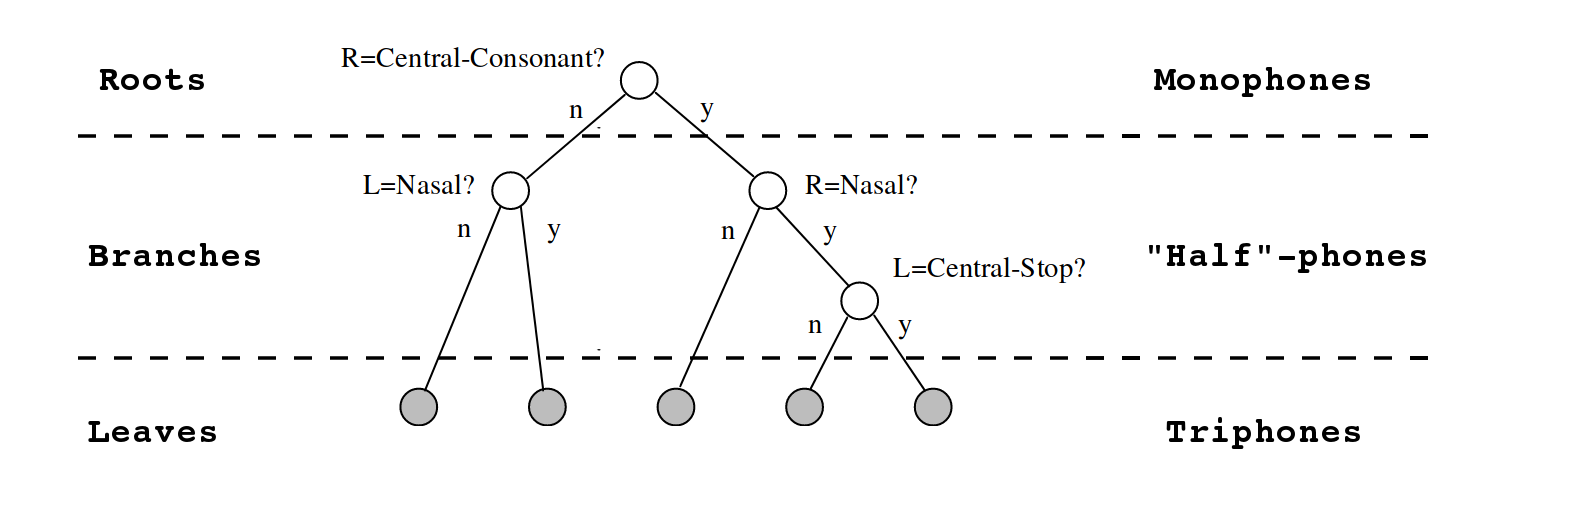
\includegraphics[width=\linewidth]{figs/levels.png}
  \caption{Logical Tree Parts}
\endminipage\hfill
\end{figure}


The ``half''-phones were created by halving the optimal number of leaves from the triphone system (ie. 1584 leaves) and re-training a new GMM-HMM system with half the optimal number of leaves (1/2 * 1584 = 792 leaves). All the other parameters were left unchanged (number of Gaussian components, iterations of EM, etc.). 


By forcing the neural net to recognize higher levels in the tree, we will learn representations which are more abstract, and therefore more likely to be relevant multi-lingually. 

Each of the following tasks were trained on the 5 hour section of LibriSpeech corpus. They are included as an extra output layer in the TDNN.

\begin{table}[!htbp]
  \centering
    \caption{Auxiliary Tasks}
  \begin{adjustbox}{width=.45\textwidth}
    \begin{tabular}{lcc}
      \toprule
      \textbf{Logical Tree Part} & \textbf{Level of Phonetic Detail} & \textbf{ \textnumero~of Tasks}\\
      \midrule
      Roots & Monophones & 1\\
      Branches & Half-phones & 1\\
      Leaves & Triphones & 1\\ 
      Lower Tree & Monophones + Half-phones & 2\\
      Upper Tree & Half-phones + Triphones & 2\\
      Whole Tree & Monophones + Half-phones + Triphones & 3\\
      \bottomrule
    \end{tabular}
    \label{table:data}
  \end{adjustbox}
\end{table}



The addition of each above task adds approximately 5 hours of training data to the standard training of a Single Task Model on Kyrgyz. As such, a weighting procedure was used to balance the relative influence of source vs. target training data on backprop. For example, to reach a one-to-one ratio, where one hour of Kyrgyz is equal to one hour of English, I multiplied every Kyrgyz gradient by $3.06$.

\begin{table}[!htbp]
  \centering
    \caption{Target:Source Data Weighting Scheme}
  \begin{adjustbox}{width=.3\textwidth}
    \begin{tabular}{cc}
      \toprule
      \textbf{Target:Source Ratio} & \textbf{Target Weight}\\
      \midrule
      1:2 & 1.53x  \\
      1:1 & 3.06x  \\
      2:1 & 6.11x  \\
      \bottomrule
    \end{tabular}
    \label{table:data}
  \end{adjustbox}
\end{table}




\subsection{Results}


All results are performed on the same held-out section of Kyrgyz audiobook. The bigram language model, lexicon, and main-task decision tree are build into a standard decoding graph in the traditional Kaldi style. Decoding is performed with a bigram backoff language model trained on a Wikipedia Kyrgyz dump, and contains, 103,998 unigrams and 56,6871 bigrams.


\begin{enumerate}
\item Addition of LibriSpeech beats out Kyrgyz-only.
\item Triphones work better than monophones
\item Both languages / tasks overfit
\item best triphone model beats best baseline (ie. early stopping)
\item atai overfit slower with additional tasks
\item atai overfits with monophones earlier, I think because it's an easier task
\item 10-to-1 weighting on 5 epochs seems like we've overfit the data, but validation is STILL increaing... try to run on 10 epochs and see what happens. 500 dim, 5 layer, aux task == triphones.
\item try 5-to-1, because 2-to-1 seems too weak, and 10-to-1 seems too strong
  \item only train on 30 minutes of Krygyz... more likely to find an effect
\end{enumerate}




\begin{table}[!htbp]
  \centering
    \caption{1-to-2 Weighting // 5-layer // 500-dim //  10 epoch }
  \begin{adjustbox}{width=.45\textwidth}
    \begin{tabular}{lc}
      \toprule
      \textbf{Auxiliary (Source Lang) Tasks} & \textbf{WER\%}\\
      \midrule
      STL Baseline &  \% \\
      Monophones &  \% \\
      Halfphones &  \% \\
      Triphones &  \%  \\
      Monophones + Halfphones & \%  \\
      Halfphones + Triphones & \%  \\
      Monophones + Halfphones + Halfphones & \%  \\
      \bottomrule
    \end{tabular}
    \label{table:data}
  \end{adjustbox}
\end{table}


\begin{table}[!htbp]
  \centering
    \caption{1-to-1 Weighting // 5-layer // 500-dim //  10 epoch }
  \begin{adjustbox}{width=.45\textwidth}
    \begin{tabular}{lc}
      \toprule
      \textbf{Auxiliary (Source Lang) Tasks} & \textbf{WER\%}\\
      \midrule
      STL Baseline &  \% \\
      Monophones &  \% \\
      Halfphones &  \% \\
      Triphones &  \%  \\
      Monophones + Halfphones & \%  \\
      Halfphones + Triphones & \%  \\
      Monophones + Halfphones + Halfphones & \%  \\
      \bottomrule
    \end{tabular}
    \label{table:data}
  \end{adjustbox}
\end{table}


\begin{table}[!htbp]
  \centering
    \caption{2-to-1 Weighting // 5-layer // 500-dim //  10 epoch }
  \begin{adjustbox}{width=.45\textwidth}
    \begin{tabular}{lc}
      \toprule
      \textbf{Auxiliary (Source Lang) Tasks} & \textbf{WER\%}\\
      \midrule
      STL Baseline &  \% \\
      Monophones &  \% \\
      Halfphones &  \% \\
      Triphones &  \%  \\
      Monophones + Halfphones & \%  \\
      Halfphones + Triphones & \%  \\
      Monophones + Halfphones + Halfphones & \%  \\
      \bottomrule
    \end{tabular}
    \label{table:data}
  \end{adjustbox}
\end{table}



\section{Discussion}


\section{Conclusions}

\section{Acknowledgements}


\bibliographystyle{IEEEtran}

\bibliography{mybib}

% \begin{thebibliography}{9}
% \bibitem[1]{Davis80-COP}
%   S.\ B.\ Davis and P.\ Mermelstein,
%   ``Comparison of parametric representation for monosyllabic word recognition in continuously spoken sentences,''
%   \textit{IEEE Transactions on Acoustics, Speech and Signal Processing}, vol.~28, no.~4, pp.~357--366, 1980.
% \bibitem[2]{Rabiner89-ATO}
%   L.\ R.\ Rabiner,
%   ``A tutorial on hidden Markov models and selected applications in speech recognition,''
%   \textit{Proceedings of the IEEE}, vol.~77, no.~2, pp.~257-286, 1989.
% \bibitem[3]{Hastie09-TEO}
%   T.\ Hastie, R.\ Tibshirani, and J.\ Friedman,
%   \textit{The Elements of Statistical Learning -- Data Mining, Inference, and Prediction}.
%   New York: Springer, 2009.
% \bibitem[4]{YourName17-XXX}
%   F.\ Lastname1, F.\ Lastname2, and F.\ Lastname3,
%   ``Title of your INTERSPEECH 2018 publication,''
%   in \textit{Interspeech 2018 -- 19\textsuperscript{th} Annual Conference of the International Speech Communication Association, September 2-6, Hyderabad, India Proceedings, Proceedings}, 2018, pp.~100--104.
% \end{thebibliography}

\end{document}
